\chapter{\ExaHyPE}
\label{section:python-api-examples:finite-volumes}


\begin{figure}[htb]
 \begin{center}
  \includegraphics[width=0.2\textwidth]{60_exahype/EU.png}
  \includegraphics[width=0.5\textwidth]{60_exahype/ExaHyPE_Logo.jpg}
 \end{center}
 \caption{
   The original ExaHyPE project delivering the first generation of the ExaHyPE
   software has received funding from the European Union’s Horizon 2020 research
   and innovation programme under grant agreement No 671698 (ExaHyPE).
 }
\end{figure}

\noindent
\ExaHyPE\ is the follow-up development of the ExaHyPE project which has been
funded by the EU from 2015--2019.
The present version is the second generation of the code (\ExaHyPE) and has
seen substantial rewrites of core routines.
However, many paradigms and even code blocks remain the same.
Migrating from the original ExaHyPE to \ExaHyPE\ thus should be straightforward.


\ExaHyPE\ is both a set of C/C++ and Fortran core routines complementing the
\Peano\ core and a high-level augmentation of \Peano's Python API.
Compare to the architecture sketch from Chapter \ref{chapter:architecture}.
\ExaHyPE's Python API can be read as builder mechanism:
You configure your particular \ExaHyPE\ application, i.e.~you tell the \ExaHyPE\
engine which application you want to run (which PDE terms, which solver
variants, which hardware properties).
The Python API then yields both a \Peano\ Python project which you can run plus
a set of template classes which you implement with your particular application.


The present document discusses how to create an \ExaHyPE\ application from
scratch.
Most application experts might not want to do this and instead use a read-to-use
\ExaHyPE\ application.
The most prominent (and maybe powerful) code using the ExaHyPE engine is maybe
ExaSeis; used to simulate seismic waves.
The details of these domain-specific codes are not covered by the present
document.



\section*{Preparing \Peano\ to run \ExaHyPE}

It is relatively straightforward to use \ExaHyPE\ within \Peano:

\begin{itemize}
  \item Configure your code with the flag \texttt{--enable-exahype}.
  \item Recompile your code. This should give you a couple of
  \texttt{ExaHyPE2Core} libraries in the respective subdirectories.
  \item Ensure that \texttt{python/exahype} is in your Python search path.
\end{itemize}


\section*{Difference of \ExaHyPE\ vs.~ExaHyPE (first generation)}

The original ExaHyPE had been built on top of Peano (third generation) and tried
to hide as much of Peano away as possible.
In \ExaHyPE, I go the opposite way: \ExaHyPE\ is a full-blown Peano add-in and I
try not to hide anything away.
Where we designed our own data management on top of Peano in ExaHyPE, all the
data management (as well as parallelisation, e.g.) is native \Peano.


With the migration from a sole-C++ philosophy to C++ supplemented by a Python
API in \Peano, I also dumped ExaHyPE's former configuration/specification file
pradigma.
An \ExaHyPE\ application now is championed by a sole Python script.
This Python script yields a native \Peano\ application (builder mechanism) which
then assembles the application.



\section{Minimalistic Finite Volumes for the Euler equations}
\label{section:exahype:fv}

We provide a complete Finite Volume implementation of a plain Euler solver
realised with \ExaHyPE. 
This solver relies on a Rusanov flux and can, with only a few lines, be
changed into an ADER-DG scheme later.
Indeed, it can be used by an ADER-DG scheme as a limiter later on.
All example data can be found within the directory
\texttt{python/examples/exahype2/finitevolumes}.


\subsection{Preparation}

Our centrel Euler script first includes a couple of tools that we need to work
with \ExaHyPE:

\begin{code}
import peano4
import peano4.datamodel
import peano4.solversteps
import peano4.output
import peano4.visualisation
import peano4.toolbox.blockstructured

import exahype2
\end{code} 


\noindent
Different to a \Peano\ application, we now do create an \ExaHyPE\ project
instance
\begin{code}
project = exahype2.Project( ["examples", "exahype2", "finitevolumes"], "finitevolumes", "." )
\end{code}
\noindent
which is assigned a subnamespace, a project name and an output path.


Next, we add the Finite Volumes solver to the project. 
This step also specifies the number of unknowns and the patch sizes that we want
to use:
\begin{code}
patch_size = 25
unknowns   = 5
project.add_finite_volumes_solver("Euler", patch_size, unknowns, 0.0001)
\end{code}
\noindent
The solver is called \texttt{Euler}.


Once this minimalist \ExaHyPE\ project is done, we ask it to generate a \Peano\
project for us, let this project parse our configure script's outcome (so that
we use the same compiler settings and other options), and we also tell \Peano\
where to find our \ExaHyPE\ libraries.
Please note that \Peano\ builds these libraries in different variants
(production runs, tracing or debugging flavours, \ldots).
Select the right one:

\begin{code}
peano4_project = project.generate_Peano4_project()
peano4_project.output.makefile.parse_configure_script_outcome( "../../../.." )
peano4_project.output.makefile.add_library( "ExaHyPE2Core2d_debug", "../../../../src/exahype2" )
peano4_project.generate(peano4.output.Overwrite.Default)
peano4_project.build()
\end{code}


\noindent
We can directly run this code (though it does nothing so far and might even
crash as we haven't set initial conditions properly) via
\begin{code}
success = peano4_project.run( [] )
\end{code}
within the Python workbench. 
Alternatively, you can invoke the code directly from the command line. 



\subsection{Implementing the Euler solver}

The run of \ExaHyPE\ so far has given us a lot of glue code (which we will
never touch) and three files in the main directory:
\texttt{AbstractEuler.h}, \texttt{Euler.h} and \texttt{Euler.cpp}.
It is the last one that we have to alter to inject our domain knowledge,
i.e.~the PDE\footnote{If you regenerate your \ExaHyPE\ code later on, it will
overwrite the Abstract\ldots solver classes, but it will never modify your
actual solver instances. So if signatures change, you will have to alter these
guys manually.}.


There are three routines that require our attention.
The first one is \texttt{adjustSolution}.
We can use this routine to overwrite the solution at any time and, hence, to
inject boundary conditions or stimuli into the domain.
It is also this routine that allows us to realise initial conditions:
\begin{code}
void examples::exahype2::finitevolumes::Euler::adjustSolution(
  double Q[5],
  const tarch::la::Vector<Dimensions,double>&  x,
  const tarch::la::Vector<Dimensions,double>&  h,
  const tarch::la::Vector<Dimensions,double>&  t
) {
  if (tarch::la::equals(t,0.0) ) {
    // initial conditions
    bool isInTheCentre = ( tarch::la::norm2( x-tarch::la::Vector<Dimensions,double>(0.5) ) < 0.05 );
    Q[0] = 1.0;  // rho
    Q[1] = 0;    // velocities
    Q[2] = 0;
    Q[3] = 0;
    Q[4] = isInTheCentre ? 1.0 : 0.0; // inner energy
  }
}
\end{code}


\noindent
As second and third step, we have to write our actual flux and eigenvalue
functions as we need them for Rusanov:

\attachfile[icon=Paperclip,description=Download code snippet,author=Peano 4]
{60_exahype/Euler-eigenvalues.cpp}

\begin{code}
void examples::exahype2::finitevolumes::Euler::eigenvalues(
  double                                       Q[5],
  const tarch::la::Vector<Dimensions,double>&  faceCentre,
  const tarch::la::Vector<Dimensions,double>&  volumeH,
  const tarch::la::Vector<Dimensions,double>&  t,
  int                                          normal,
  double                                       lambda[5]
) {
  [...]
}
\end{code}



\attachfile[icon=Paperclip,description=Download code snippet,author=Peano 4]
{60_exahype/Euler-flux.cpp}


\begin{code}
void examples::exahype2::finitevolumes::Euler::flux(
  double                                       Q[5],
  const tarch::la::Vector<Dimensions,double>&  faceCentre,
  const tarch::la::Vector<Dimensions,double>&  volumeH,
  const tarch::la::Vector<Dimensions,double>&  t,
  int                                          normal,
  double                                       F[5]
) {
  [...]
}
\end{code}


\noindent
There are quite a lot of assertions in the code in the repository that you might
want to skip (and I didn't paste them in here).
I found them useful when I wrote \ExaHyPE\ in the first place.
With these implementations in place, you can finally type in \texttt{make} in
the project directory and rerun the code.
Alternatively, just re-execute the whole Python script.
You'll get your first wave equation solver

Some simple boundary conditions close the system:

\begin{code}
void examples::exahype2::finitevolumes::Euler::boundaryConditions(
  double                                       Qinside[5],
  double                                       Qoutside[5],
  const tarch::la::Vector<Dimensions,double>&  faceCentre,
  const tarch::la::Vector<Dimensions,double>&  volumeH,
  const tarch::la::Vector<Dimensions,double>&  t,
  int                                          normal
) {
  Qoutside[0] = Qinside[0];
  Qoutside[1] = Qinside[1];
  Qoutside[2] = Qinside[2];
  Qoutside[3] = Qinside[3];
  Qoutside[4] = Qinside[4];
}
\end{code}



\subsection{Configuring the overall run}

\ExaHyPE's Python interface gives you the opportunity to specify exactly which
domain you want to use, how often to plot, and when to shut down the simulation.
For a first trial, we set the parameters as follows:
\begin{code}
project.set_global_simulation_parameters(
  2,         # Dimensions
  [0.0,0.0], # Offset of computational domain
  [1.0,1.0], # Size of computational domain
  0.2,       # Terminal time, i.e. we simulate from 0 to 0.2
  0.0,       # First snapshot of solution is done after grid construction, i.e. at time 0
  0.001      # We then plot every 0.001 time units
)
\end{code}
\noindent
This is all. We now can run the code.


\subsubsection{IO and logging}


\ExaHyPE\ codes by default yield snapshots in \Peano's block format. 
If you have configured \Peano\ with VTK support, you can directly convert it
into VTK and visualise through Paraview or VisIt, e.g.:
\begin{code}
if success:
  convert = peano4.visualisation.Convert( "solutionEuler" )
  convert.set_visualisation_tools_path( "../../../../src/visualisation" )
  convert.extract_fine_grid()
  convert.convert_to_vtk()
\end{code}


\ExaHyPE\ searches for a text file \texttt{exahype.log-filter} in the working
directory.
If no such file is found (or the file is corrupted), then it will use some
default filter rules, i.e.~dump the information to the terminal that I consider
to be most important.
If you want to adopt the output, I strongly recommend that you add a log filter
configuration file. 
The syntax of log filter files is discussed in Section
\ref{section:logging:log-filter}.



\subsection{Running on a parallel computer}

To run \ExaHyPE\ in parallel, you have to build \Peano\ with support for
multithreading and/or MPI.
Once this is done, the engine more or less runs in parallel out of the box.


\paragraph{Domain decomposition}
The core domain decomposition scheme realised in \ExaHyPE\ is a non-overlapping
multiscale domain decomposition based upon space-filling curves (SFC).
To use this scheme, you have to specify an appropriate load balancing scheme.
Without any load balancing, the code will never split up the domain and thus
effectively run serially.

\begin{figure}
 \begin{center}
  \includegraphics[width=0.54\textwidth]{60_exahype/domain-decomposition.png}
 \end{center}
 \caption{
  Domain decomposition in \ExaHyPE\ for a run with four threads/ranks. Each
  individual cell hosts a patch.
 }
\end{figure}


I plan to support multiple different dynamic load balancing schemes over time,
but the straightforward decomposition scheme shipped with \Peano\ at the moment
is recursive subdivision, a modification of OpenMP's guided scheduling.
To use it, you have to call
\begin{code}
project.set_load_balancing( "toolbox::loadbalancing::RecursiveSubdivision" )
\end{code}

\noindent
on your \ExaHyPE\ project. You can add  


\paragraph{Task decomposition}
\ExaHyPE\ realises an additional task decomposition working on top of the domain
decomposition. 
This task decomposition is shared memory, only.
That is, you can use task decomposition without domain decomposition, but then
you won't benefit from multiple nodes.
You can however always use domain decomposition without task
decomposition---though it should be slower in most cases.

\begin{remark}
This section is under construction.
\end{remark} 





\section{Finite Volumes with ClawPack (ExaClaw)}

ExaClaw is an extension of \ExaHyPE\ (Chapter \ref{chapter:exahype}) which
offers the ClawPack Riemann solvers within \ExaHyPE.
Its development has been made possible by EPSRC under the Excalibur
Phase I call.
The grant number is EP/V00154X/1.


\begin{remark}
 This solver family is work-in-progress.
\end{remark}



\section{Ghoddess DG solvers}

We also do provide an interface to Ghoddess DG solvers.
Ghoddess solvers use a classic DG formulation with explicit time stepping.
Their big USP within \ExaHyPE\ is they rely on a quasi-symbolic formulation and
thus facilitate even fast prototyping.

\begin{remark}
 Add copyright et al here.
\end{remark}

\subsection{Preparation}

We first install Ghoddess:

\begin{remark}
 Add instructions here.
\end{remark}


\subsection{Using the Ghoddess solver}

From hereon, our description follows the Finite Volume example from Section
\ref{section:exahype:fv}, i.e.~we only highlight where we do things differently.
Besides our \ExaHyPE\ modules, we first include the ghoddess subpackage which is
not by default included:

\begin{code}
import os
import peano4
import exahype2
import exahype2.ghoddess
\end{code} 

From hereon, we create the Ghoddess solver and add it to the project:

\begin{code}
project = exahype2.Project( ["examples", "exahype2", "advection"], "ghoddess", "." )
order          = 23
unknowns       = 5
time_step_size = 0.0001
project.add_solver(  exahype2.ghoddess.RusanovLegendreWithFixedTimeStepSize(
  "Advection", order, unknowns, 0.0001) )
\end{code}


\subsection{Using the Ghoddess solver}

\begin{remark}
 This part has yet to be written. Have no clue how we do this.
\end{remark}


\section{Introducing a new numerical scheme}

This section discusses how to introduce a totally new numerical solver. 
It does not discuss how to introduce a new PDE, as new PDEs are built on top of
\ExaHyPE.
This section gives you an idea how to extend \ExaHyPE\ instead.

\begin{remark}
  \ExaHyPE\ is a very high level Python API which generates a \Peano\
   Python project which in turn creates the ``real'' \Peano\ C/C++ code. If you
   introduce a new numerical scheme/solver to \ExaHyPE, you thus might want to
   familiarise yourself with \Peano's Python API and how to extend it. This
   recommendation affects all the gluecode/framework aspects of the software.
   All the core numerics of \ExaHyPE\ are held as C++ code in the
   \texttt{src/exahype2} directly and compiled into a separate library. If you
   introduce new numerical schemes, you might have to extend this library, too.
\end{remark}



\subsection{A new Finite Volume solver (native \ExaHyPE)}

Introducing a new Finite Volume scheme is reasonably straightforward within
\ExaHyPE.
It relies directly on \Peano's patch-based AMR.


\begin{itemize}
  \item Create a new subclass of \texttt{exahype2.solver.FV}. The parent class
  has to be told with which patch overlaps you work.
  \item Instantiate this class in your user code when you invoke
  \texttt{add\_solver} on the \ExaHyPE\ project.
  \item Overwrite \texttt{get\_user\_includes()} to add all the includes for
  C/C++ code that you'll eventually need. 
  \item If you class is called \texttt{XYZ}, create four text files:
  \texttt{XYZAbstract.template.h}, \linebreak \texttt{XYZAbstract.template.cpp},
  \texttt{XYZ.template.h} and \texttt{XYZ.template.cpp}.
\end{itemize}

\noindent
\ExaHyPE's design concept is that each solver yields two types of classes:
The actual solver and an abstract superclasses. 
Abstract superclasses are regenerated every time you rerun the Python script.
Furthermore, they define the whole signature, i.e.~if you alter the signature
later on, users simply rerun the toolkit. 
Finally, the abstract superclasses hold default implementations.


With \Peano, you can create arbitrary abstract superclasses. 
They have to implement some general \ExaHyPE\ routines, but the number of operations that they have to
provide is very small.
I thought about introducing a general \texttt{exahype2::Solver} class, but then
this class is not really required anywhere as we work with code generation all
the way through anyway. 
So the only thing your solver's abstract superclass has to give \ExaHyPE\ is the
following set of routines:

\begin{code}
  double getMinTimeStamp() const;
  double getMaxTimeStamp() const;
  double getMinTimeStepSize() const;
  double getMaxTimeStepSize() const;

  void startTimeStep(
      double globalMinTimeStamp,
      double globalMaxTimeStamp,
      double globalMinTimeStepSize,
      double globalMaxTimeStepSize
  );

  void finishTimeStep();
\end{code}
\noindent
You can make them virtual if you want to highlight that a user can reimplement
them. 
But there's no need for this. 


The core implementation effort clearly has to go into the parts where the actual
mesh traversal is mapped onto solver calls.
In \ExaHyPE, this is realised through templates. 
Any user solver is supposed to define three local variables within its solver
class:
\texttt{HandleBoundaryTemplate}, 
\texttt{CreateCellTemplate}, \texttt{HandleCellTemplate} and
\texttt{AMRTemplate}.
There are more, but this is the minimum.


Within these templates, you have access to a couple of variables, some symbols,
and you can furthermore specify your own replacement rules:
\begin{itemize}
  \item Within each code block, you have access to a variable marker which is of
  type \texttt{peano4::datamanagement::FaceMarker} or
  \texttt{peano4::datamanagement::CellMarker}. It allows you to find out more
  about the face or cell centre, mesh sizes, \ldots, i.e.~it holds all spatial
  information.
  \item Within each code block, the constant \texttt{\{SOLVER\_INSTANCE\}} will
  be replaced by the Python code with an actual instance of your user's solver.
  \item The constant
  \texttt{\{NUMBER\_OF\_VOLUMES\_PER\_AXIS\}} will be replaced by the block size
  specified by the user. It is the attribute you hand through in the
  constructor.
  \item The constant
  \texttt{\{NUMBER\_OF\_UNKNOWNS\}} will be replaced by the argument you pass to
  the constructor.
  \item There are more constants. See \linebreak
  \texttt{peano4.solvers.FV.\_\_init\_dictionary\_with\_default\_parameters} for
  information.
  \item You can introduce more symbolds as \texttt{\{XYZ\}} as long as you add
  them within your routine
  \texttt{add\_entries\_to\_text\_replacement\_dictionary}.
\end{itemize}


\noindent
The template mechanism works similar to aspect-oriented programming, i.e.~it
simply enables Python to plug some code snippets straight into your the
generated \ExaHyPE\ code. 
The interesting thing however is the symbol

\begin{itemize}
  \item \texttt{fineGridCell\{UNKNOWN\_IDENTIFIER\}.value} which is a double
    pointer which points to the whole patch hosted by the cell in the volumetric
    routines \texttt{CreateCellTemplate}, \texttt{HandleCellTemplate} and
    \texttt{AMRTemplate}. The array it points to has the size \linebreak
    \texttt{\{NUMBER\_OF\_VOLUMES\_PER\_AXIS\}}$^d \cdot $
    \texttt{\{NUMBER\_OF\_UNKNOWNS\}}.
  \item \texttt{fineGridFace\{UNKNOWN\_IDENTIFIER\}.value} is the face
    equivalent for the boundary conditions. Again, it is a double pointer,
    though one dimension is not equal to
    \texttt{\{NUMBER\_OF\_VOLUMES\_PER\_AXIS\}} but equal to the halo overlap.
    See the Finite Volumes discussion in
    Chapter~\ref{section:python-api-examples:finite-volumes}.
  \item \texttt{reconstructedPatch} and \texttt{originalPatch} are only defined
    within \texttt{HandleCellTemplate}. The former is an alias for
    \texttt{fineGridFace\{UNKNOWN\_IDENTIFIER\}.value}, i.e.~points to the same
    location. \texttt{reconstructedPatch} is another pointer which points to the
    patch from the previous mesh traversal, i.e.~you can overwrite data
    within \texttt{originalPatch} and still have the old one available.
    Furthermore, the underlying patch is bigger: It hosts the actual patch data
    plus its halo.
\end{itemize}




\begin{remark}
 If you want to see a really simple example of this solver type, change into the 
 directory \texttt{src/exahype2/fv} and have a look into \texttt{Rusanov.cpp}.
 It follows exactly the above recipe.
\end{remark}


\noindent
I see two different ways how to realise a new solver: 
You can either code your solver directly within the Python templates.
Alternatively, you can generate some generic glue code within the template and
forward calls to some predefined C++ or user code.


Both variants have pros and cons and are valid.
For my generic Rusanov solver (as well as for ADER-DG), we can realise all
numerics generically within predefined kernels relying only on few user-defined
functions injecting flux and eigenvalues.
Furthermore, these functions have the same signature for all applications.
For a bespoke Finite Volume scheme where the Riemann solver holds the actual
numerical wisdom and each Riemann solvers requires a bespoke signature, it is
maybe better to skip that additional level of abstraction.



\subsection{Ghoddess implementation remarks}

Ghoddess works on triangles which we embed into the squares or cubes,
respectively, of \ExaHyPE.
By default, the code employs Gauss-Legendre sample points.
The data structure used thus read as follows
(Fig.~\ref{figure:60_exahype:degree-of-freedom-layout:Ghoddess}):
\begin{itemize}
  \item The solver embeds a ``patch'' of $N$ polynomial weights into each cell.
  For order $p=1, d=2$, we have for example $N=6$, for $p=2, d=2$ we have
  $N=12$.
  \item Each face carries $2(p+1)^{d-1}$ doubles.
\end{itemize}


\noindent
The face data holds a left and a right representation of the polynomial along
the face.
So it does not really hold degrees of freedom.
Its degree of freedom are mere projections of the cell solution onto the face.



\begin{figure}
 \begin{center}
  \includegraphics[width=0.65\textwidth]{60_exahype/Ghoddess-dof-layout.pdf}
 \end{center}
 \caption{
  Left: Degree of freedom layout in Ghoddess within a cell.
  Right: Each face holds additional ``degree of freedoms'' which encode the
  projection of the cell polynomial onto the face.
  \label{figure:60_exahype:degree-of-freedom-layout:Ghoddess}
 }
\end{figure}

The Ghoddess solver itself splits up into four computation kernels:

\begin{enumerate}
  \item The {\bf projectOntoFace} kernel accepts the $N$ degrees of freedom from
  the cell and projects the polynomials of the two triangles within the cell
  onto the faces. It consequently writes $2d \cdot (p+1)^{d-1}$ face DoFs. Once
  we have traversed the whole mesh, each face ``knows'' its left and right
  projection.
  \item The {\bf solveRiemann} kernel takes the $2 \cdot (p+1)^{d-1}$ DoFs on
  the face, i.e.~the left and right projection, and solves the Riemann problem
  on the jump. The result is written back into the $2 \cdot (p+1)^{d-1}$ DoFs.
  In principle, this allows us to have a different outgoing flux for the left
  and right side of a face.
  \item The {\bf solveCell} kernel evolves the solution within the triangle
  pair, i.e.~it evaluates the volumetric integrals of the DG formulation. The
  name is slightly wrong: Besides the volumetric terms, the kernel also
  evaluates the face terms arising between the two triangles embedded into the
  cell. So it is a combination of a cell kernel plus one Riemann solve (in 2d).
  \item The {\bf projectOntoCell} kernel takes the Riemann solution on the cell
  faces, i.e.~the output of projectOntoFace, and adds it to the cell solution,
  i.e.~it adds it to the outcome of solveCell.
\end{enumerate}


\noindent
Ghoddess' vanilla version indeed traverses the mesh four times per time step.
This makes it easy/easier to debug the code and to analyse the substeps.
The work of Charrier et al then automatically fuses the traversals and thus
reduces the memory accesses and homogenises the computational character over the
mesh sweeps.


The realisation of the four sweeps relies on blockstructured extension of
\Peano:
Though the data is logically not Cartesian or block-structured, we model all
properties as blocks embedded into the mesh.


All solvers inherit from \texttt{exahype2.ghoddess.Solver} which is our abstract
framework.
Per solver, the Python API will generate one C++ solver class.
This class has a couple of things to do:

\begin{enumerate}
  \item It holds all time stepping data. So it knows, for example, what the
  minimal time stamp at the moment is.
  \item It serves as a state machine which decides at any point which kernels
  are to be executed on particular grid entities.
  \item It holds the application domain-specific routines such as the actual
  kernel implementations, refinement criteria or data initialisation.
\end{enumerate}



\section*{Links and further reading}

\begin{itemize}
  \item The ``official'' ExaHyPE release paper is
{\tiny \begin{verbatim}
@article{Reinarz:2019:ExaHyPE,   
  title = "ExaHyPE: An engine for parallel dynamically adaptive simulations of wave problems",
  journal = "Computer Physics Communications",
  pages = "107251",
  year = "2020",
  issn = "0010-4655",
  doi = "https://doi.org/10.1016/j.cpc.2020.107251",
  url = "http://www.sciencedirect.com/science/article/pii/S001046552030076X",
  author = "Anne Reinarz and Dominic E. Charrier and Michael Bader and Luke Bovard and Michael Dumbser 
    and Kenneth Duru and Francesco Fambri and Alice-Agnes Gabriel and Jean-Matthieu Gallard and 
    Sven Köppel and Lukas Krenz and Leonhard Rannabauer and Luciano Rezzolla and Philipp Samfass and 
    Maurizio Tavelli and Tobias Weinzierl",
  keywords = "Hyperbolic, PDE, ADER-DG, Finite volumes, AMR, MPI, TBB, MPI+X",
}
  \end{verbatim}}
  If you use the software, it would be great if you could cite this one.
\end{itemize}

